\documentclass[aps,prl,reprint]{revtex4-1}
\usepackage[utf8]{inputenc}
\usepackage{gensymb}
\usepackage{float}
\usepackage[spanish]{babel}
\usepackage{graphicx}
\usepackage{babel}
\begin{document}
\title{Laboratorio Microondas}

\author{Daniel Fajardo}
\author{Juan Sebastian Vargas}
 \affiliation{Universidad de los Andes, Departamento de f\'isica}
 

\date{18 de febrero de 2016}

\setlength{\columnsep}{1.5cm}





\begin{abstract}
    
La radiación electromagnética, que esta compuesta por ondas electromagnéticas, fue descubierta en los inicios del siglo 19. Las Microondas son ampliamente utilizadas en telecomunicaciones, radares y muchos usos mas. En este experimento se utilizo un emisor de microondas con $\lambda= 2.85 cm$ con el cual se observaron varios fenómenos de las ondas E.M.\\
\textit{Palabras clave: Radiación Electromagn\'etica, Microondas, Campos El\'ectrico, Campo Magnetico, Polarización}


\end{abstract}
\maketitle

\section{Introducci\'on}
    SE DEBE HACER UN MARCO TEORICO DE:
    ONDAS ELECTROMAGNETICAS, POLARIZACION, RESULTADOS ESPERADOS DE LOS EXPERIMENTOS \\
La Polarizacion es un vector que apunta en la misma dirección que  $\vec{E}$ y se denota como: $\vec{n}$

\section{Montaje Experimental}

El primer montaje consiste colocar el emisor frente al recibidor, y variar la distancia entre los dos como se muestra en la figura \ref{monta1}:\\
\begin{figure}[h]
 \scalebox{0.4}{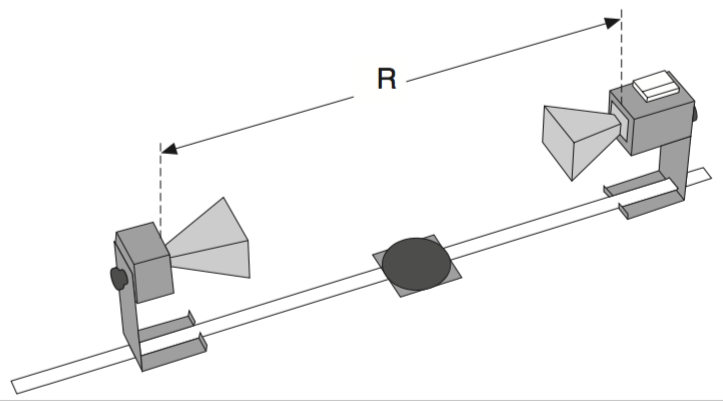
\includegraphics{monta1.png}} 
 \caption{Primer montaje}
 \label{monta1}
\end{figure}


Donde se varia la distancia $R$ y se anota su respectivo valor de intensidad dado por el recibidor. Se hizo la medición para 7 diferentes valores de $R$ con valores entre $40 cm$ hasta $100 cm$. Ademas con el mismo montaje de la Figura \ref{monta1} dejando un $R$ constante  se roto el recibidor cada $10\degree$ empezando en su posición natural ($0\degree$) hasta $180\degree$




\section{Resultados y An\'alisis}
En la Tabla \ref{tbmonta1.1} podemos ver la relación entre la distancia $R$ y la intensidad relativa medida por el recibidor:\\

\begin{table}[H]
\begin{center}

\begin{tabular}{|| r || c ||} 
\hline\hline
R(cm) & Medicion (mA) \\ \hline
40             & \textgreater 1        \\ \hline
50             & 0.86              \\ \hline
60             & 0.65              \\ \hline
70             & 0.50              \\ \hline
80             & 0.36              \\ \hline
90             & 0.2               \\ \hline
100            & 0.14              \\ \hline

\end{tabular}
\end{center}
\caption{Tabla que muestra la medicion con su respectivo valor de R}
\label{tbmonta1.1}
\end{table}


\begin{figure}[H]
 \scalebox{0.5}{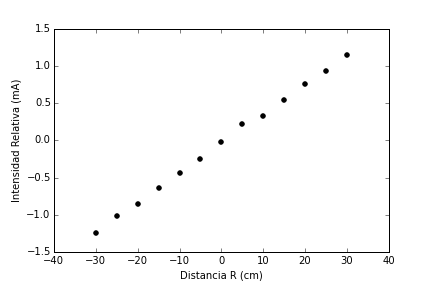
\includegraphics{grmonta1_1.png}} 
 \caption{Grafico de la intensidad contra distancia}
 \label{gmonta1.1}
\end{figure}


En la Figura \ref{gmonta1.1} vemos una grafica de los puntos de la Tabla \ref{tbmonta1.1} y a simple vista se puede ver que la intensidad medida es inversamente proporcional a la distancia, resultado que no nos sorprende ya que la intensidad disminuye con la distancia.

Cuando dejamos $R$ constante y rotamos el recibidor obtenemos la siguiente tabla:

\begin{table}[H]
\begin{center}

\begin{tabular}{|| r || c ||} 
\hline\hline
Angulo Recibidor(\degree) & Medicion (mA) \\ \hline
0             & 1        \\ \hline
10             & 1              \\ \hline
20             & 0.95              \\ \hline
30             & 0.84              \\ \hline
40             & 0.70              \\ \hline
50             & 0.52              \\ \hline
60            & 0.28             \\ \hline
70 & 0.07 \\ \hline
80 & 0 \\ \hline
90 & 0 \\\hline
100 & 0 \\ \hline
110 & 0 \\ \hline
120 & 0.04 \\ \hline
130 & 0.37 \\ \hline
140 & 0.58 \\ \hline
150 & 0.77 \\ \hline
160 & 0.92 \\ \hline
170 & 1 \\ \hline
180 & \textgreater 1 \\ \hline

\end{tabular}
\end{center}
\caption{Tabla de la variacion de la Intensidad en funci\'on del angulo}
\label{tbmonta1.2}
\end{table}

\begin{figure}[H]
 \scalebox{0.5}{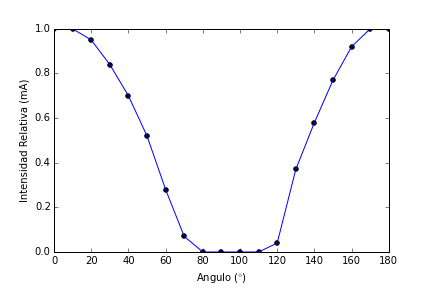
\includegraphics{grmonta1_2.png}} 
 \caption{Grafico de Intensidad contra Angulo de rotacion}
 \label{gmonta1.2}
\end{figure}
En la Figura \ref{gmonta1.2} obtenemos un resultado esperado, ya que el emisor genera ondas que tienen polarización lineal, cuando el vector $\vec{n}$ se encuentra en la misma dirección que la polarización del recibidor ($0\degree$) la intensidad será máxima, ya que las polarizaciones coincides, cuando este ángulo va cambiando la intensidad disminuye, hasta el punto en el que la Intensidad es mínima cuando $\vec{n}$ es perpendicular a la polarización del recibidor($90\degree$).


\section{Conclusiones}



\end{document}